\documentclass[11pt]{amsart}
%prepared in AMSLaTeX, under LaTeX2e
\addtolength{\oddsidemargin}{-.5in} 
\addtolength{\evensidemargin}{-.5in}
\addtolength{\topmargin}{-.25in}
\addtolength{\textwidth}{1.2in}
\addtolength{\textheight}{0.95in}

\renewcommand{\baselinestretch}{1.08}

\usepackage{fancyvrb} % for "comment" environment

\newcommand{\mfile}[1]{
\begin{quote}
\bigskip
\VerbatimInput[frame=single,label=\fbox{\normalsize \textsl{\,#1\,}},fontfamily=courier,fontsize=\scriptsize]{#1}
\end{quote}
}

\usepackage{hyperref}
\usepackage{xspace}

\newtheorem*{thm}{Theorem}
\newtheorem*{defn}{Definition}
\newtheorem*{example}{Example}
\newtheorem*{problem}{Problem}
\newtheorem*{remark}{Remark}

\usepackage[final]{graphicx}


% macros
\usepackage{amssymb}
\newcommand{\bA}{\mathbf{A}}
\newcommand{\bB}{\mathbf{B}}
\newcommand{\bE}{\mathbf{E}}
\newcommand{\bF}{\mathbf{F}}
\newcommand{\bJ}{\mathbf{J}}
\newcommand{\br}{\mathbf{r}}
\newcommand{\bx}{\mathbf{x}}
\newcommand{\hbi}{\mathbf{\hat i}}
\newcommand{\hbj}{\mathbf{\hat j}}
\newcommand{\hbk}{\mathbf{\hat k}}
\newcommand{\hbn}{\mathbf{\hat n}}
\newcommand{\hbr}{\mathbf{\hat r}}
\newcommand{\hbt}{\mathbf{\hat t}}
\newcommand{\hbx}{\mathbf{\hat x}}
\newcommand{\hby}{\mathbf{\hat y}}
\newcommand{\hbz}{\mathbf{\hat z}}
\newcommand{\hbphi}{\mathbf{\hat \phi}}
\newcommand{\hbtheta}{\mathbf{\hat \theta}}
\newcommand{\complex}{\mathbb{C}}
\newcommand{\ppr}[1]{\frac{\partial #1}{\partial r}}
\newcommand{\ppt}[1]{\frac{\partial #1}{\partial t}}
\newcommand{\ppx}[1]{\frac{\partial #1}{\partial x}}
\newcommand{\ppy}[1]{\frac{\partial #1}{\partial y}}
\newcommand{\ppz}[1]{\frac{\partial #1}{\partial z}}
\newcommand{\pptheta}[1]{\frac{\partial #1}{\partial \theta}}
\newcommand{\ppphi}[1]{\frac{\partial #1}{\partial \phi}}
\newcommand{\Div}{\ensuremath{\nabla\cdot}}
\newcommand{\Curl}{\ensuremath{\nabla\times}}
\newcommand{\curl}[3]{\ensuremath{\begin{vmatrix} \hbi & \hbj & \hbk \\ \partial_x & \partial_y & \partial_z \\ #1 & #2 & #3 \end{vmatrix}}}
\newcommand{\cross}[6]{\ensuremath{\begin{vmatrix} \hbi & \hbj & \hbk \\ #1 & #2 & #3 \\ #4 & #5 & #6 \end{vmatrix}}}
\newcommand{\eps}{\epsilon}
\newcommand{\grad}{\nabla}
\newcommand{\image}{\operatorname{im}}
\newcommand{\integers}{\mathbb{Z}}
\newcommand{\ip}[2]{\ensuremath{\left<#1,#2\right>}}
\newcommand{\lam}{\lambda}
\newcommand{\lap}{\triangle}
\newcommand{\note}[1]{[\scriptsize #1 \normalsize]}
\newcommand{\MatIN}[1]{\mtt{>> #1}}
\newcommand{\onull}{\operatorname{null}}
\newcommand{\rank}{\operatorname{rank}}
\newcommand{\range}{\operatorname{range}}
\renewcommand{\P}{\mathcal{P}}
\newcommand{\real}{\mathbb{R}}
\newcommand{\trace}{\operatorname{tr}}

\renewcommand{\Re}{\operatorname{Re}}
\renewcommand{\Im}{\operatorname{Im}}
\newcommand{\Arg}{\operatorname{Arg}}

\newcommand{\pf}{\textsc{Proof}.\xspace}

\newcommand{\Matlab}{\textsc{Matlab}\xspace}
\newcommand{\Octave}{\textsc{Octave}\xspace}
\newcommand{\MO}{\textsc{Matlab/Octave}\xspace}

\newcommand{\ppart}[1]{\textbf{(#1)}\, }
\newcommand{\epart}[1]{\medskip\noindent\quad\textbf{(#1)}\, }
\newcommand{\prob}[1]{\medskip\noindent\textbf{#1.}\quad }



\begin{document}
\scriptsize \noindent Math 310 Numerical Analysis, Fall 2012 (Bueler) \hfill \today
\normalsize\bigskip
\thispagestyle{empty}

\Large

\centerline{\textbf{Solutions to Assignment \#2}}
\normalsize

\medskip

\prob{1} \ppart{a} The Vandermonde system of equations is
\begin{align*}
a_0 + a_1 + a_2 &= 1 \\
a_0 + 2.5 a_1 + (2.5)^2 a_2 &= 8 \\
a_0 + 4 a_1 + 4^2 a_2 &= 5
\end{align*}
Entered into \MO:
\small \begin{quote}\begin{Verbatim}
>> A = [1 1 1; 1 2.5 2.5^2; 1 4 4^2];
>> b = [1 8 5]';
>> v = A \ b
v =
     -9.2222
      12.444
     -2.2222
\end{Verbatim}
\end{quote} \normalsize
Thus the polynomial is $P(x) = -9.2222 + 12.444\, x - 2.2222\, x^2$.

\epart{b} In the Newton form we start with the unknown polynomial $P(x) = c_0 + c_1(x-1) + c_2(x-1)(x-2.5)$.  Then the system of equations looks like
$$\begin{array}{lcl}
c_0      &=& 1 \\
c_0 + 1.5 c_1    &=& 8 \\
c_0 + 3 c_1 + 4.5 c_2  &=& 5
\end{array}$$
Again in \MO, and reusing the same \texttt{b}:
\small \begin{quote}\begin{Verbatim}
>> M = [1 0 0; 1 1.5 0; 1 3 4.5];
>> w = M \ b
w =
           1
      4.6667
     -2.2222
\end{Verbatim}
\end{quote} \normalsize
Thus the polynomial is $P(x) = 1 + 4.6667 (x-1) - 2.2222 (x-1)(x-2.5)$.

\epart{c} The Lagrange polynomials are, in turn:
\begin{align*}
\ell_1(x) &= \frac{(x-2.5)(x-4)}{(1-2.5)(1-4)} = \frac{2}{9} (x-2.5)(x-4), \\
\ell_2(x) &= \frac{(x-1)(x-4)}{(2.5-1)(2.5-4)} = - \frac{4}{9} (x-1)(x-4), \\
\ell_3(x) &= \frac{(x-1)(x-2.5)}{(4-1)(4-2.5)} = \frac{2}{9} (x-1)(x-2.5).
\end{align*}
Thus the polynomial is
\begin{align*}
   P(x) &= 1\,\ell_1(x) + 8\,\ell_2(x) + 5\,\ell_3(x) \\
        &= \frac{2}{9} (x-2.5)(x-4) - \frac{32}{9} (x-1)(x-4) + \frac{10}{9} (x-1)(x-2.5)
\end{align*}

\epart{d} Tedious but straightforward calculations show that the answers to \textbf{(b)} and \textbf{(c)} are identical to that in \textbf{(a)}, once they are put in monomial (standard) polynomial form.  Another way to check that these are all the same results is to plot:
\small \begin{quote}\begin{Verbatim}
>> x = 0:.01:5;
>> plot([1 2.5 4],[1 8 5],'ko')
>> hold on
>> plot(x,-9.2222 + 12.444*x - 2.2222*x.^2,'b')
>> plot(x,1 + 4.6667*(x-1) - 2.2222*(x-1).*(x-2.5),'g')
>> plot(x,(2/9)*(x-2.5).*(x-4) - (32/9)*(x-1).*(x-4) + (10/9)*(x-1).*(x-2.5),'r')
>> hold off
\end{Verbatim}
\end{quote} \normalsize
You'll see one parabolic curve, which happens to be in red because that was our last color, and with black circles at the three points we claimed to pass through.


\prob{2}  I wrote the following code:

\mfile{randsixpoly.m}

One particular run is shown in figure 1; at the command line:

\begin{figure}[ht]
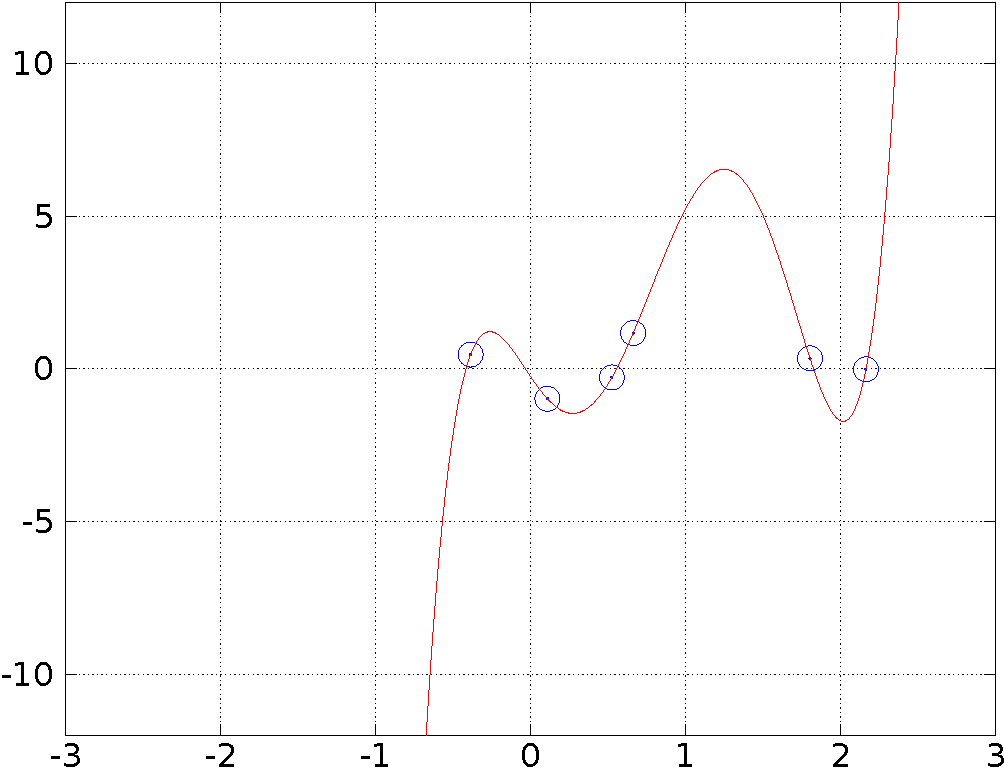
\includegraphics[width=0.5\textwidth]{randsixpoly}
\caption{A typical polynomial of degree 5 going through 6 random points.}
\end{figure}

\small \begin{quote}\begin{Verbatim}
>> randsixpoly
result:
  P(x) = -0.235985 + -7.532621 x + 4.110836 x^2 + 34.791169 x^3 +
         + -34.268908 x^4 + 8.348005 x^5
\end{Verbatim}
\end{quote} \normalsize
Your answer will \emph{not} be the same.

In fact, because the code generates random points, it produces a new output every time you run it.  This can be a disadvantage, because it is harder to test for correctness if you do not have repeatability.  To get repeatability, one simple way is to compute the random points \emph{once} and then hard-code those numbers into the m-file.  Another is to ``seed'' the (pseudo-)random number generator.  For example, consider the commands:
\small \begin{quote}\begin{Verbatim}
>> rand('seed',12.3456789)
>> rand
\end{Verbatim}
\end{quote} \normalsize
The second command will always produce the same result because the first command fixes the ``seed'' the same way each time.

Now, I did not ask you if finding this polynomial \emph{was a good idea}.  If you have six data points, should you put a degree five polynomial through this data?  Generally, should high degree polynomials be put through data points?  \emph{NO}!

Said more carefully, if the points are not the values of a \emph{smooth} and \emph{precisely-known} function then you should \emph{not} use high-degree polynomial interpolation.  The interpolating polynomial will generally not be similar to the function ``behind your data.''  Instead, low degree polynomial \emph{regression}, for instance linear regression, is likely to be a good idea if the the points are imperfect data.   That is, inexactly fitting a low degree polynomial to the data, in the sense of least squares, is better than exactly fitting the data by using a high degree polynomial.


\prob{3} \emph{The solution method for lower triangular systems is very natural: start at the first equation and get the unknowns in turn.}

\epart{a} I solved the system by hand: $x=3$, $y=-1$, $z=-7/3$.

\epart{b}  The solution is straightforward to write, as long as it is understood that you \emph{must use these equations in the order they are given}.  That is, as unknowns $x_j$ become known, they can be used in the next equation:
\begin{align*}
x_1 &= \frac{b_1}{a_{11}} \\
x_2 &= \frac{b_2 - a_{21} x_1}{a_{22}} \\
& \vdots \\
x_j &= \frac{b_j - a_{j1} x_1 - a_{j2} x_2 - \dots - a_{j,j-1} x_{j-1}}{a_{jj}} \\
 & \vdots \\
x_n &= \frac{b_n - a_{n1} x_1 - a_{n2} x_2 - \dots - a_{n,n-1} x_{n-1}}{a_{nn}}
\end{align*}

This system is solvable if all $a_{jj}$ are nonzero.  In that case there is a unique solution.


\prob{4}  \ppart{a} \ppart{b} \ppart{c} I wrote the following code which does all three parts.  The result is in left side of figure 2.

\mfile{smoothpolyapprox.m}

\begin{figure}[ht]
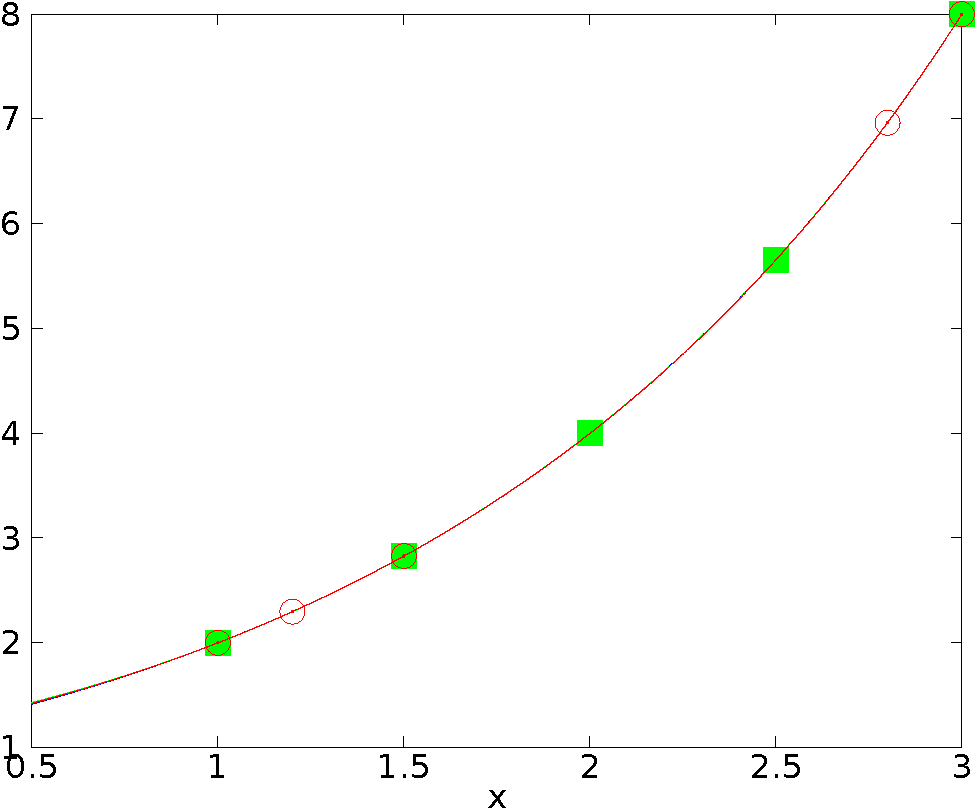
\includegraphics[width=0.46\textwidth]{smoothpolyapprox} \, 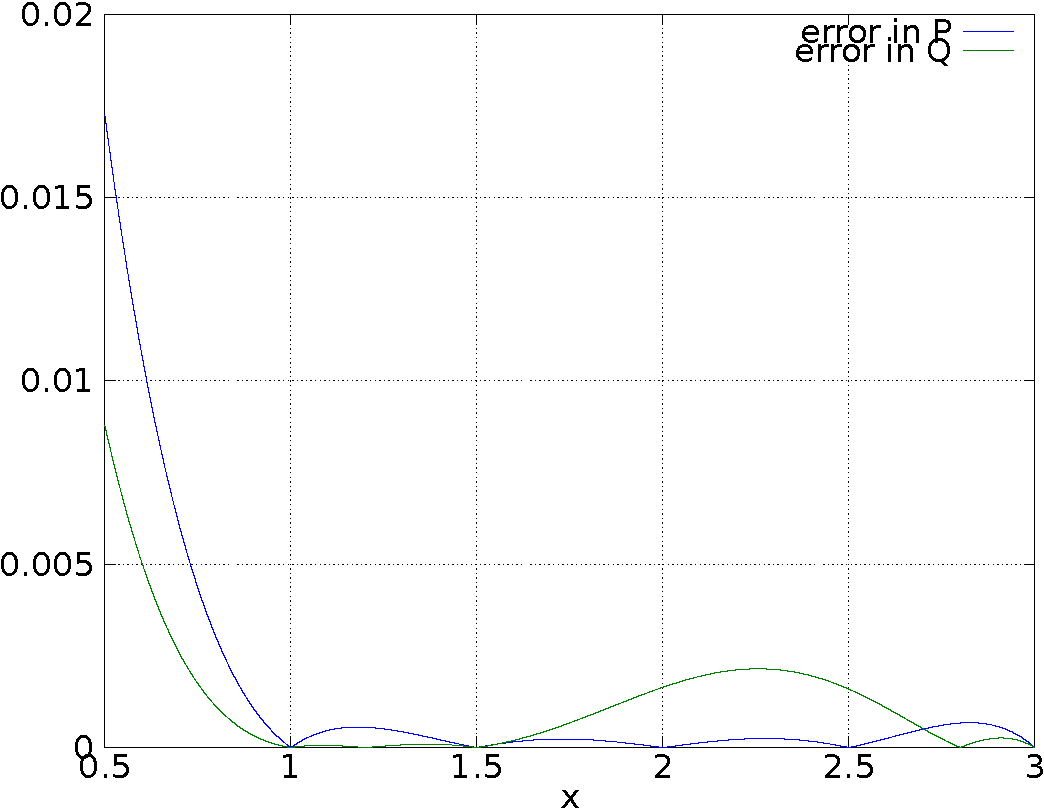
\includegraphics[width=0.49\textwidth]{clearpolyerror}
\caption{\textbf{Left.}  Degree four polynomials interpolating $y=2^x$ on the interval $[0.5,3]$.  They do an excellent job.  At screen resolution we cannot tell the difference between the three curves $y=2^x$, $y=P(x)$, and $y=Q(x)$.  The green squares show the interpolation points for $P$ and the red circles show the points for $Q$.  \textbf{Right.} Computing differences shows some differences in the location and magnitude of the error.}
\end{figure}

The left part of Figure 2 raises the question: are these polynomial interpolants equally good?  Any assessment of the quality of the interpolant is answered by graphing the differences:
\small\begin{quote}\begin{Verbatim}
>> figure, plot(xx,abs(2.^xx-P),xx,abs(2.^xx-Q)), grid on, xlabel x
>> legend('error in P','error in Q')
\end{Verbatim}
\end{quote}\normalsize
This is shown in the right side of Figure 2.

\end{document}
